\documentclass{article}
\usepackage{graphicx} % Required for inserting images
\usepackage{babel}[polish]
\usepackage{polski}
\usepackage{float}
\usepackage{adjustbox}
\usepackage{subfig}
\usepackage{booktabs}
\usepackage{siunitx}
\usepackage[a4paper,top=2cm,bottom=2cm,left=3cm,right=3cm,marginparwidth=1.75cm]{geometry}
\usepackage{tikz}
\usepackage{pgfplots}
\usepackage{pgfplotstable}
\usepackage{amsmath}
\usepackage{filecontents}
\usepackage{wrapfig}
\usepackage{svg}
\usepackage{tabularx}
\usepackage{array}
\newcolumntype{Y}{>{\centering\arraybackslash}X}
\usepackage{xcolor,colortbl}
\usepackage{pdfpages}

\pgfplotsset{compat=newest}
\usepgfplotslibrary{external}
\tikzexternalize[prefix=tikz/]

\title{ELA2 - Projekt}
\author{Piotr Pokornowski 325061}
\date{\today}

\begin{document}

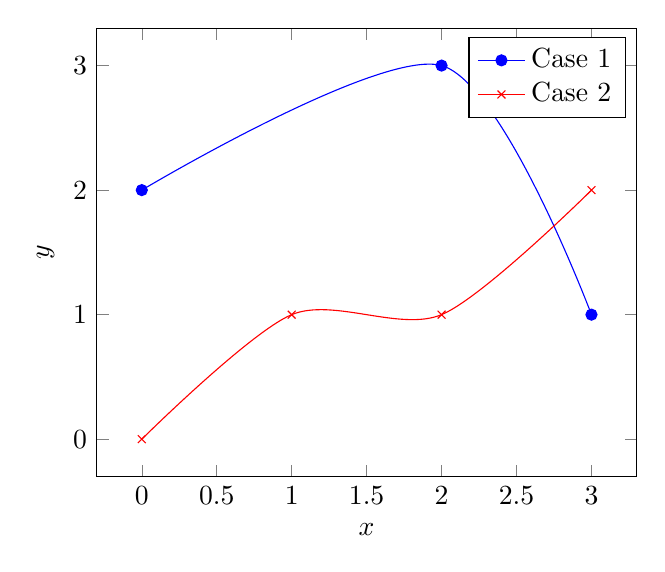
\begin{tikzpicture}
    \begin{axis}[
            xlabel=$x$,
            ylabel=$y$]
        \addplot[smooth,mark=*,blue] plot coordinates {
                (0,2)
                (2,3)
                (3,1)
            };
        \addlegendentry{Case 1}

        \addplot[smooth,color=red,mark=x]
        plot coordinates {
                (0,0)
                (1,1)
                (2,1)
                (3,2)
            };
        \addlegendentry{Case 2}
    \end{axis}
\end{tikzpicture}
\end{document}


% \begin{tikzpicture}
%     \begin{axis}[
%             %axis background/.style={fill=black},
%             grid=both,
%             xlabel={$t$},
%             ylabel= { $V_{\text{OUT}}$ },
%             ymin=-1,
%             ymax=6,
%             xmin=0,
%             xmax=0.008,
%             ytick distance=1,
%             xtick distance=0.001,
%             tick label style={font=\tiny},
%             title={\SI{5}{\V} / \SI{5}{\A}},
%         ]
%         %\addplot[color=green] table {./figures/digital/vout/segment_1.csv};
%         %\addplot[color=green] table {./figures/digital/vout/segment_1.csv};
%         \label{plot:vout} % Label for vout plot
%     \end{axis}

%     % Adding extra y-axis for current
%     \begin{axis}[
%             axis y line*=right,
%             axis x line=none,
%             ymin=-1,
%             ymax=6,
%             ytick pos=right,
%             yticklabel pos=right,
%             ytick distance=1,
%             ylabel={$I_{\text{OUT}}$},
%             tick label style={font=\tiny},
%         ]
%         %\addplot[color=red] table {./figures/digital/iout/segment_1.csv};
%         %\addplot[color=red] table {./figures/digital/iout/segment_2.csv};
%         \label{plot:current} % Label for current plot
%     \end{axis}
% \end{tikzpicture}
% \label{fig:subfig2}